\documentclass[11pt,a4paper]{article}

\usepackage[T1]{fontenc}
\usepackage[utf8]{inputenc}
\usepackage{lmodern}
\usepackage{microtype}
\usepackage{amsmath}
\usepackage[margin=2.6cm]{geometry}
\usepackage{booktabs}
\usepackage{tabularx}
\usepackage{graphicx}
\usepackage{caption}
\usepackage{float}
\usepackage{xcolor}
\usepackage{fancyhdr}
\usepackage[hidelinks]{hyperref}

\definecolor{accent}{HTML}{275CB2}
\definecolor{notebg}{HTML}{F1F5FB}
\hypersetup{colorlinks=true, linkcolor=accent, urlcolor=accent}
\captionsetup{font=small, labelfont={bf,color=accent}, width=0.92\textwidth}

\pagestyle{fancy}
\fancyhf{}
\renewcommand{\headrulewidth}{0.4pt}
\fancyhead[L]{\footnotesize\sffamily Project 3 --- Active Learning for Learning-to-Defer}
\fancyhead[R]{\footnotesize\sffamily Kartik Anand, 676049}
\fancyfoot[C]{\footnotesize\thepage}

\setlength{\parskip}{0.55em}
\setlength{\parindent}{0pt}
\renewcommand{\arraystretch}{1.15}
\setlength{\emergencystretch}{2.5em}

\makeatletter
\renewcommand\section{\@startsection{section}{1}{\z@}%
  {-3.5ex \@plus -1ex \@minus -.2ex}{2.2ex \@plus.2ex}%
  {\normalfont\Large\sffamily\bfseries\color{accent}}}
\renewcommand\subsection{\@startsection{subsection}{2}{\z@}%
  {-3.0ex \@plus -1ex \@minus -.2ex}{1.4ex \@plus .2ex}%
  {\normalfont\large\sffamily\bfseries\color{accent}}}
\renewcommand\paragraph{\@startsection{paragraph}{4}{\z@}%
  {2.4ex \@plus1ex \@minus.2ex}{-0.8em}%
  {\normalfont\normalsize\sffamily\bfseries\color{black}}}
\makeatother

\newsavebox{\calloutbuf}
\newenvironment{callout}
  {\par\medskip\begin{lrbox}{\calloutbuf}%
   \begin{minipage}{\dimexpr\linewidth-24pt\relax}\setlength{\parskip}{0.4em}}
  {\end{minipage}\end{lrbox}%
   \noindent\colorbox{notebg}{\hspace{4pt}\usebox{\calloutbuf}\hspace{4pt}}\par\medskip}

\newcommand{\file}[1]{\texttt{\small #1}}

\title{\vspace{-1.4cm}\sffamily\color{accent}\bfseries
       Active Learning for Learning-to-Defer\\[0.25em]
       \Large\mdseries Project 3 --- Human-Centric Artificial Intelligence}
\author{Kartik Anand \quad---\quad Matriculation 676049\\[0.3em]
        \small Hamburg University of Technology \quad SoSe 2026}
\date{\small \today}

\begin{document}
\maketitle
\thispagestyle{fancy}

\begin{callout}
A classifier that is right 92.3\,\% of the time is paired with a simulated expert
who is right only 69.9\,\% of the time. Deciding, per article, which of the two
should answer raises the pair to 94.1\,\% while consulting the expert on 16\,\%
of articles. This report describes how that decision is learned, how it is
measured, and how the expert's competence can be discovered from a few hundred
questions rather than from complete knowledge.
\end{callout}

\tableofcontents
\vspace{1em}

% ============================================================================
\section{Setting}

The dataset is AG News: 120{,}000 training and 7{,}600 test articles, exactly
balanced across four topics (World, Sports, Business, Sci/Tech). Each article is
a headline and a short snippet, median 232 characters.

The system may answer an article itself or defer it to a human expert. Deferring
is not free --- it costs a person's attention --- and it is not always
beneficial, because the expert is sometimes worse than the machine. The problem
is to learn where deferring pays.

Everything is scikit-learn, numpy and matplotlib. No neural networks, no
pretrained embeddings. All expensive work is precomputed by
\file{manage.py prepare\_project3} and cached, because the interface must not
spend minutes on a page load.

% ============================================================================
\section{Task 1 --- The classifier}

TF-IDF over word unigrams and bigrams, sublinear term frequency, minimum document
frequency 2, capped at 50{,}000 features, followed by multinomial logistic
regression with $C = 4$.

\textbf{Test accuracy: 0.9233.}

\subsection{Why this one}

Four candidates were measured on the real data:

\begin{center}
\small
\begin{tabular}{@{}lrr@{}}
\toprule
\textbf{Model} & \textbf{Test accuracy} & \textbf{Fit time} \\
\midrule
1--2gram TF-IDF + LinearSVC ($C = 0.5$)        & 0.9287 & 19\,s \\
1--2gram TF-IDF + logistic regression ($C = 4$) & 0.9241 & 55\,s \\
1gram TF-IDF + logistic regression              & 0.9171 & 18\,s \\
1--2gram TF-IDF + ComplementNB                  & 0.9092 & 13\,s \\
\bottomrule
\end{tabular}
\end{center}

LinearSVC is the most accurate and was rejected anyway. It reports a decision
value, not a calibrated probability, and every part of Tasks 3 and 4 depends on
knowing \emph{how confident} the classifier was rather than merely what it
guessed. Section~\ref{sec:confidence} shows that confidence turns out to be the
single most informative feature in the whole project, which makes 0.46 points of
accuracy a cheap purchase.

Feature count was decided the same way. At 300{,}000 features the model scores
0.9241 and pickles to 21.9\,MB; at 50{,}000 it scores 0.9233 and pickles to
3.6\,MB. Eight ten-thousandths of accuracy for a sixfold smaller artefact is
worth taking when the deployment target has 512\,MB of memory. Hashing features
were also tried and were worse on both axes (0.9120, 10.5\,MB).

\subsection{Out-of-fold scoring, which everything downstream depends on}

Tasks 3 and 4 need to know where the classifier is wrong on the \emph{training}
set, because that is the training signal for the competence models. Scored on its
own training data the classifier makes 3{,}403 mistakes; scored 5-fold
out-of-fold it makes 11{,}350.

\begin{callout}
Using the in-sample figure would have understated classifier failure by a factor
of 3.3 and taught the deferral model that the classifier almost never needs help.
The error is silent --- nothing crashes, the numbers merely come out wrong --- so
all downstream targets use the out-of-fold predictions, which are cached
alongside the model.
\end{callout}

% ============================================================================
\section{Task 2 --- The simulated experts}

\subsection{The invariant}

The brief requires experts that are imperfect and that ``exhibit expertise in
specific regions of the input space''. One constraint was imposed on top of that,
and it determines everything else:

\begin{callout}
\textbf{An expert's competence is a function of the input only, never of the true
label.}

Task 4 has to discover the competence profile by querying, and at query time the
true label is precisely what is unknown. An expert defined as ``reliable whenever
the true topic is Sports'' cannot be discovered by any honest procedure, because
predicting their competence would require already knowing the answer. Task 4
would be vacuous by construction.
\end{callout}

The one place the true label is used is choosing \emph{which} wrong answer to
give when the expert errs. That is a property of the simulation and not of the
competence: nothing downstream predicts the content of a wrong answer, only
whether an answer is right.

\subsection{Expert A --- specialist desks}

$k$-means with $K = 12$ partitions the TF-IDF training matrix into regions. Five
of the twelve, fixed by a recorded seed, are the expert's beat. Inside them they
are correct with probability 0.95; outside, 0.40. Wrong answers are drawn
uniformly from the other three topics.

\textbf{Test accuracy: 0.6988}, i.e. 22 points below the classifier.

\begin{figure}[H]
\centering
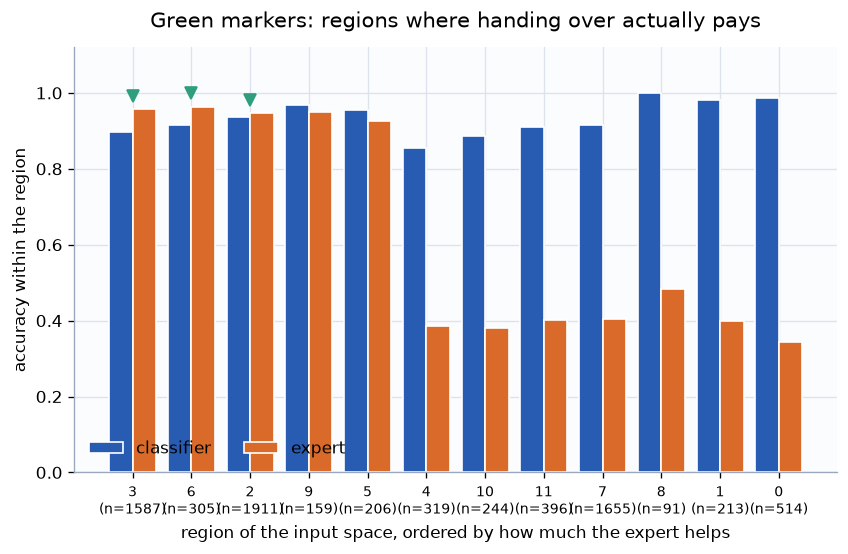
\includegraphics[width=0.92\textwidth]{figures/p3-desks-regions.png}
\caption{Expert and classifier accuracy within each region, ordered by how much
the expert helps. Green markers show the regions where deferring actually pays.}
\label{fig:desks-regions}
\end{figure}

\paragraph{Strengths and weaknesses.} The interesting part of
Figure~\ref{fig:desks-regions} is not that the expert is strong in five regions
--- that was constructed --- but that being strong is not sufficient. In one
specialist region the expert scores 0.931 while the classifier scores 0.969, so
deferring there \emph{loses} accuracy despite the region being the expert's own
subject. Only three of the twelve regions are worth deferring in once the
classifier's own strength is accounted for.

This is why the region table in the interface reports both accuracies side by
side rather than the expert's alone. An analysis that showed only where the
expert is good would recommend deferring in a region where deferring is harmful.

\subsection{Expert B --- headline reader}

A contrast, not a better idea. Competence varies smoothly with three surface
properties --- text length, digit density, and the proportion of capitalised
tokens --- and is deliberately unrelated to subject matter.

\textbf{Test accuracy: 0.6814.}

Its purpose is to test whether the Task 4 results describe a method or one lucky
competence structure. Section~\ref{sec:task4} reports that they do not fully
generalise, which is the reason for including it.

% ============================================================================
\section{Task 3 --- Learning to defer}

\subsection{The rule}

Two logistic regressions, each estimating a probability of being correct:
\[
  m_{\text{clf}}(x) = P(\text{classifier right} \mid x), \qquad
  m_{\text{exp}}(x) = P(\text{expert right} \mid x).
\]
Neither predicts the topic. Both predict whether an answer would be correct,
which is a different and harder question. The system defers when
\[
  m_{\text{exp}}(x) - m_{\text{clf}}(x) > \tau ,
\]
with $\tau$ exposed to the user as a cost-of-interruption control rather than
fixed in code, because its right value depends on how expensive the expert's time
is relative to a mistake --- a judgement no analysis can make on the user's
behalf.

\subsection{The feature representation}
\label{sec:confidence}

Both heads are fitted on a 100-component truncated SVD of the TF-IDF matrix plus
three numbers describing the classifier's own confidence: its top probability,
the gap between its top two, and its entropy.

Including confidence explicitly is not tidying. Measured on the training set:

\begin{center}
\small
\begin{tabular}{@{}lrr@{}}
\toprule
\textbf{Predictor of ``is the classifier right?''} & \textbf{AUC} & \textbf{Dimensions} \\
\midrule
Top-two margin alone            & 0.8476 & 1 \\
All TF-IDF features alone       & 0.8006 & 50{,}000 \\
TF-IDF + confidence             & 0.8710 & 50{,}003 \\
SVD-100 + confidence            & 0.8552 & 103 \\
\bottomrule
\end{tabular}
\end{center}

A single number --- how close the classifier's top two guesses were --- predicts
its own correctness better than all fifty thousand word features put together.
When a model is unsure, it is usually unsure for a reason.

The compact representation was chosen over the full one deliberately. It costs
0.016 AUC, and it is what makes Task 4 possible at all: fitting a logistic
regression with $n = 200$ queried points and $d = 50{,}000$ features fits noise,
while $d = 103$ is estimable.

\subsection{Evaluation}

The brief asks that evaluation reflect ``not only classification accuracy but
also the quality of the deferral decisions''. Accuracy alone rewards a policy
that hands everything to a competent expert while having learned nothing, so
every article is placed in one of four cases:

\begin{center}
\small
\begin{tabularx}{0.94\textwidth}{@{}lX@{}}
\toprule
\textbf{Case} & \textbf{What deferring does} \\
\midrule
Only the expert is right      & the one case worth deferring \\
Both are right                & harmless, but a person's time spent for nothing \\
Only the classifier is right  & actively makes the answer worse \\
Neither is right              & harmless and pointless \\
\bottomrule
\end{tabularx}
\end{center}

From that: \textbf{deferral precision} is the share of deferred articles falling
in the first case, and \textbf{deferral recall} is the share of all first-case
articles that were actually deferred. Neither can be gamed alone --- perfect
recall by deferring everything, near-perfect precision by deferring almost
nothing --- so both are reported.

\subsection{Results}

\begin{table}[H]
\centering
\small
\begin{tabular}{@{}lrrrr@{}}
\toprule
\textbf{Policy} & \textbf{Team accuracy} & \textbf{Deferral rate} & \textbf{Precision} & \textbf{Recall} \\
\midrule
Never defer (classifier alone)          & 0.9233 & 0.000 & --- & 0.000 \\
Always defer (expert alone)             & 0.6988 & 1.000 & 0.054 & 1.000 \\
Defer the classifier's least confident  & 0.9254 & 0.164 & --- & --- \\
\textbf{Learned policy} ($\tau = -0.02$) & \textbf{0.9405} & 0.164 & 0.189 & 0.576 \\
Oracle (knows both answers)             & 0.9770 & 0.054 & 1.000 & 1.000 \\
\bottomrule
\end{tabular}
\caption{Expert A. The learned policy gains 1.72 points over the classifier
alone, at the same deferral rate as the confidence baseline, which gains only
0.21. The oracle marks 5.37 points of available headroom, of which the learned
policy captures roughly a third.}
\label{tab:defer}
\end{table}

The confidence baseline is the comparison that matters. Deferring whatever the
classifier is least sure about requires no expert data at all and is the first
thing anyone would try; at the same rate of interruption it captures 0.21 points
against the learned policy's 1.72.

\begin{figure}[H]
\centering
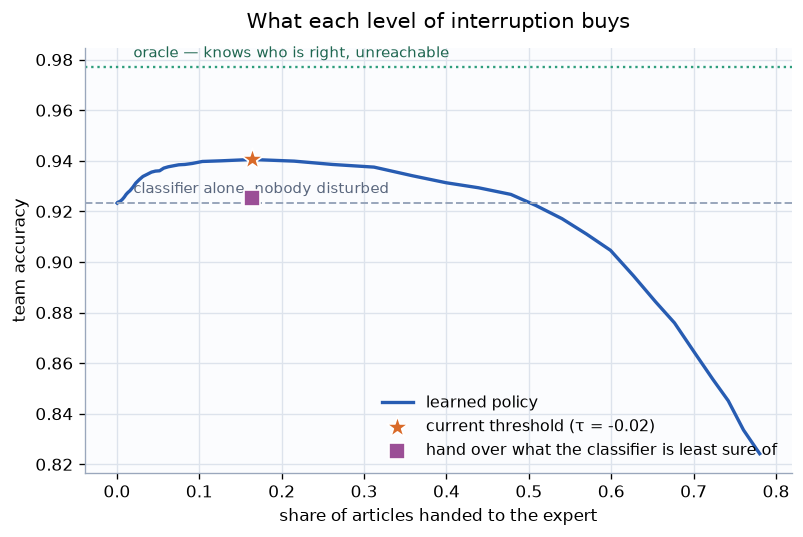
\includegraphics[width=0.86\textwidth]{figures/p3-desks-tradeoff.png}
\caption{Team accuracy against the share of articles handed to the expert.}
\label{fig:tradeoff}
\end{figure}

\begin{figure}[H]
\centering
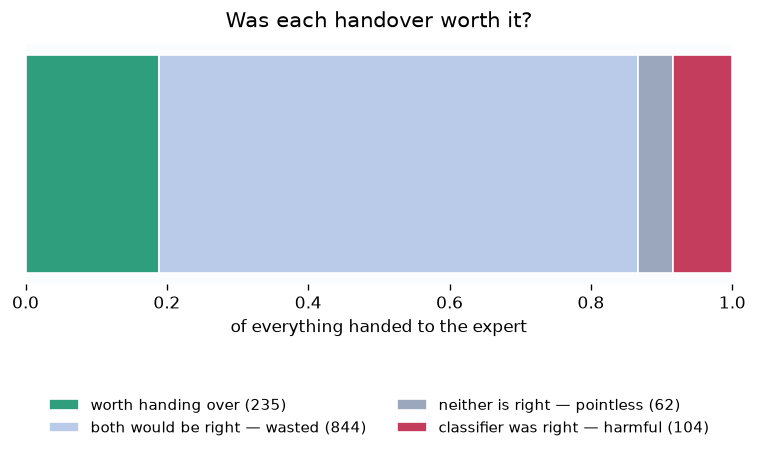
\includegraphics[width=0.86\textwidth]{figures/p3-desks-outcomes.png}
\caption{Of everything sent to the expert, only the green band needed to be sent.
Deferral precision is 0.189: most interruptions are cases both would have got
right. This is invisible in the accuracy figure and is exactly what the brief
means by the quality of the decisions.}
\label{fig:outcomes}
\end{figure}

A note against over-claiming: precision of 0.189 means roughly four in five
interruptions were unnecessary. The policy is worth having because the fifth one
rescues an answer, but a deployment where expert time was scarce would want a
much higher $\tau$ and would accept a smaller gain.

% ============================================================================
\section{Task 4 --- Active learning}
\label{sec:task4}

\subsection{The setting, and why the obvious strategy is wrong}

Now no expert answers are available. The classifier may still use the whole
labelled training set --- and, importantly, $m_{\text{clf}}$ costs nothing,
because classifier correctness is known everywhere from the out-of-fold pass. The
only unknown is $m_{\text{exp}}$, and every data point for it costs one question.

\begin{callout}
\textbf{The choice:} query the articles where the deferral decision is closest to
flipping, i.e.\ where $|m_{\text{exp}}(x) - m_{\text{clf}}(x)|$ is smallest.

\textbf{The justification:} ordinary active learning queries where the classifier
is uncertain, because the classifier is what is being learned. That does not
transfer. Here the classifier is fixed and its competence is already known for
free. A query is only worth spending if it might change the \emph{answer} to
``who should handle this article''. An article that baffles the classifier is
worth asking about only if the expert might do better; if both are lost, learning
that teaches nothing about where to defer.
\end{callout}

Classifier-entropy sampling --- the instinct this problem invites --- is
implemented as a baseline so the claim can be tested rather than asserted.

\paragraph{Cold start.} With no answers there is no $m_{\text{exp}}$ and so no
boundary to sit near. Worse, an estimate fitted on a handful of points would
confidently aim the search at the wrong place and keep it there, choosing where to
look using the very belief it is trying to correct. The first 120 queries are
therefore drawn stratified across the twelve regions, guaranteeing coverage before
targeting begins. All four strategies share this opening batch, which is why they
coincide at the left of Figure~\ref{fig:curves}.

\subsection{Results}

\begin{figure}[H]
\centering
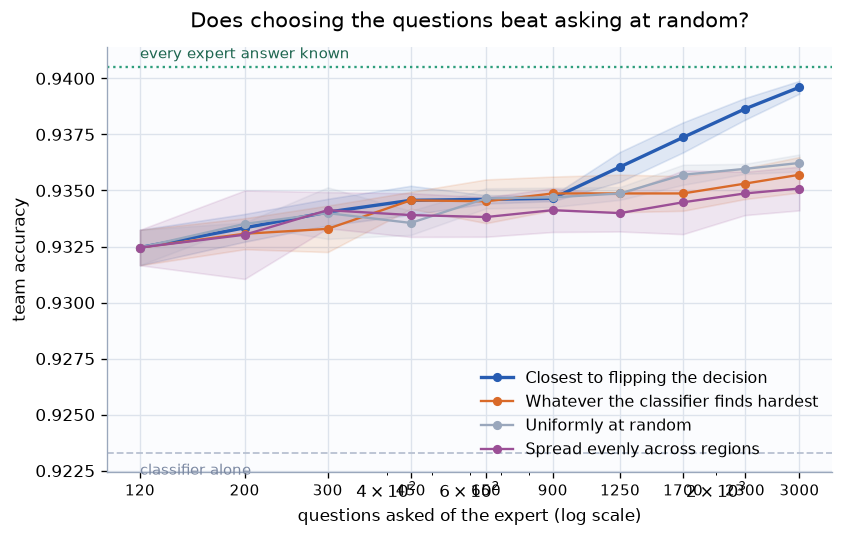
\includegraphics[width=0.86\textwidth]{figures/p3-desks-curves.png}
\caption{Expert A. Team accuracy against the number of questions asked, averaged
over three seeds; bands are one standard deviation.}
\label{fig:curves}
\end{figure}

\begin{center}
\small
\begin{tabular}{@{}lrr@{}}
\toprule
\textbf{Strategy} & \textbf{Expert A} & \textbf{Expert B} \\
\midrule
Deferral boundary (ours)      & \textbf{0.9396} & 0.9275 \\
Classifier entropy            & 0.9357 & 0.9279 \\
Uniform random                & 0.9362 & 0.9280 \\
Region-stratified random      & 0.9351 & 0.9276 \\
\midrule
Every expert answer known     & 0.9405 & 0.9300 \\
\bottomrule
\end{tabular}
\end{center}

\paragraph{Expert A.} Boundary sampling beats random by 0.0034 at 3{,}000
queries, against a run-to-run standard deviation of about 0.0004 --- roughly
eight standard deviations, so a real effect. It reaches 0.9396 against the
0.9405 obtainable with all 120{,}000 expert answers: \textbf{2.5\,\% of the
possible questions recover 96\,\% of the benefit.} Classifier entropy does indeed
underperform, finishing marginally below uniform random.

\paragraph{The result does not appear early.} Up to roughly a thousand queries
all four strategies are indistinguishable, and the gap opens only afterwards.
This is the opposite of the usual account of active learning, where the benefit
is largest when data is scarcest. The explanation is the cold-start problem
above: targeting requires an estimate good enough to aim with, and until roughly a
thousand answers have accumulated the boundary estimate is too noisy to be worth
following. Reporting this honestly matters more than the headline number.

\paragraph{Expert B --- a null result.} No strategy separates from random. The
spread across all four is smaller than the seed-to-seed variation. Expert B's
competence depends on surface properties of the text that are close to
independent of whether the classifier is right, so there is very little
structure linking the two, and no acquisition function can find structure that is
not there. The full-information ceiling is correspondingly low: 0.9300 against
Expert A's 0.9405.

\begin{callout}
The honest conclusion is narrower than ``choosing questions beats asking at
random''. It is: \emph{choosing questions helps when the expert's competence is
visible in the features the deferral model can see, and not otherwise.} Expert B
exists in this project precisely so that this boundary could be found rather than
assumed.
\end{callout}

% ============================================================================
\section{The human-centric argument}

Three things are the user's to decide, and the interface makes each of them a
control rather than a constant.

\textbf{The threshold} is the main one. Nobody can choose it analytically,
because it encodes how expensive an interruption is against how expensive a
mistake is. Moving it in the interface changes the four outcome counts
immediately, so the cost of a low threshold --- articles taken from a machine
that would have been right --- is visible rather than aggregated away. At
$\tau = -0.20$ the team is \emph{worse} than the classifier alone
($-0.0062$), which is worth being able to see.

\textbf{Which expert} is being modelled, so the user can observe that the method
works for one competence structure and not the other rather than being told a
single number.

\textbf{What is reported.} Team accuracy alone would present the policy far more
favourably than the outcome breakdown does. Showing that four in five
interruptions were unnecessary is the part a person deciding whether to deploy
this would actually need.

% ============================================================================
\section{Reproducing this}

\begin{center}
\small
\begin{tabularx}{0.94\textwidth}{@{}lX@{}}
\toprule
\textbf{File} & \textbf{Contents} \\
\midrule
\file{data.py}          & AG News, shipped as gzipped CSV with the app. \\
\file{expert.py}        & The two simulated experts and the region analysis. \\
\file{deferral.py}      & Competence heads, the deferral rule, the four-case evaluation. \\
\file{acquisition.py}   & The four query strategies and the budget simulation. \\
\file{prepare.py}       & Everything expensive, cached by \file{manage.py prepare\_project3}. \\
\file{explain.py}       & Eighteen plain-language explanations linked from the interface. \\
\bottomrule
\end{tabularx}
\end{center}

All randomness is seeded. Active learning curves are averaged over three seeds
and reported with their standard deviation; single-seed differences smaller than
about 0.001 in team accuracy should not be believed.

\end{document}
